%!TEX root = ../../Heun_Dale_Haney_A_dynamic_approach_to_input_output_modeling.tex
%%%%%%%%%%%%%%%%%%%%% chapter.tex %%%%%%%%%%%%%%%%%%%%%%%%%%%%%%%%%
%
% sample chapter
%
% Use this file as a template for your own input.
%
%%%%%%%%%%%%%%%%%%%%%%%% Springer-Verlag %%%%%%%%%%%%%%%%%%%%%%%%%%
%\motto{Use the template \emph{chapter.tex} to style the various elements of your chapter content.}
\motto{Essentially, all models are wrong, but some are useful.~\emph{\cite[p.~424]{Box:1987aa}}

\hfill---\emph{George E. P. Box}}


%%%%%%%%%%%%%%%%%%%%%%%%%%%%%%%%%%
%%%%%%%%%% Introduction %%%%%%%%%%
%%%%%%%%%%%%%%%%%%%%%%%%%%%%%%%%%%
\chapter{Accounting for the wealth of nations}
% Always give a unique label
\label{chap:acct_for_won}
% use \chaptermark{}
% to alter or adjust the chapter heading in the running head
\chaptermark{Wealth of nations}
%%%%%%%%%%%%%%%%%%%%%%%%%%%%%%%%%%
%%%%%%%%%%%%%%%%%%%%%%%%%%%%%%%%%%
%%%%%%%%%%%%%%%%%%%%%%%%%%%%%%%%%%


%% \abstract{Each chapter should be preceded by an abstract (10--15 lines long) that summarizes the content. The abstract will appear \textit{online} at \url{www.SpringerLink.com} and be available with unrestricted access. This allows unregistered users to read the abstract as a teaser for the complete chapter. As a general rule the abstracts will not appear in the printed version of your book unless it is the style of your particular book or that of the series to which your book belongs.\newline\indent
%% Please use the 'starred' version of the new Springer \texttt{abstract} command for typesetting the text of the online abstracts (cf. source file of this chapter template \texttt{abstract}) and include them with the source files of your manuscript. Use the plain \texttt{abstract} command if the abstract is also to appear in the printed version of the book.}

%% Use the template \emph{chapter.tex} together with the Springer document class SVMono (monograph-type books) or SVMult (edited books) to style the various elements of your chapter content in the Springer layout.

\abstract*{In this chapter, we describe
the development of 
approaches to the relationship between the economy and the
biosphere. 
The historical development takes place
over three eras, the era of abundance, the 
era of energy constraints, and the age of 
resource depletion. 
Each era is defined by a dominant
metaphor that guides the economic model and
leads to a framework for national accounting that is perceived 
as relevant to understanding the economy. 
The metaphor for the economy has evolved from 
the clockwork mechanism of classical physics 
(economy isolated from the environment) 
to an engine (the economy is dependent on an
inexhaustible supply of inputs from the environment).
The chapter then suggests that the previous metaphors
are insufficient for the age of resource depletion
and suggests a new metaphor: the economy is
society's \emph{metabolism}. 
Next, the way in which the metabolism metaphor leads to
an expanded understanding of the requirements
for national accounting is described.
An argument is made for
accounting a nation's wealth (manufactured 
and natural capital) in addition to its income (GDP). 
The chapter ends with a description 
of the structure of the rest of the book.
}


The Introduction (Chapter~\ref{chap:intro}) opened with
(a) the observation that economic growth has slowed
in mature economies of the world and
(b) the forecast that growth will remain slow for the foreseeable future. 
This is seen as a problem, 
because robust economic growth is thought to be a necessary condition
for maintaining growth in living standards.
The observation and forecast are widely shared among mainstream economic analysts 
who blame stagnation in the conventional factors of production 
(manufactured capital, labor, and technology---all endogenous to the economy) 
for the bleak situation. 
Proposed solutions to this economic problem include
investment in manufactured capital and technology (supply-side policies) 
or boosting consumption (demand-side policies).

We also 
presented evidence for an additional, 
biophysical reason for the slowdown:
the economy is tightly coupled to the biosphere,
and we are depleting stocks of natural capital,
particularly stores of energy.
As these natural resources are depleted,
they become more expensive to produce, and
economic growth suffers.
We suggested the startling notion that 
because standard economic theory 
does not perceive the slowdown in biophysical terms, 
the mainstream prescription of 
investment in manufactured capital could fail
as it locks in future demand for natural resources 
that become ever more expensive to extract.
Thus, policy prescriptions based on the conventional wisdom can, 
unwittingly, exacerbate economic slowdown in the long-term.

How could it be that mainstream, growth-targeted
economic policies actually contribute to slowdown?
Could it be that the mainstream model is incomplete 
or ill-suited for the age of resource depletion?

Before exploring these questions, we note that 
models (economic and otherwise) are informed by metaphors,
simplified ways of explaining and framing the world in which we live.
Looking back, we note that the Introduction (Chapter~\ref{chap:intro})
contained much metaphorical language.%
	\footnote{  %chktex 42
	The use of mechanical metaphor language in Chapter~\ref{chap:intro} 
	was deliberate decision to bring attention 
	to the dominant metaphors of the day.
	}
We spoke of 
``driving'' economic growth
and of ``fueling'' the ``economic engine.''
And, we said that the economy has ``stalled.''
Society's manner of speaking about the economy 
reveals that the dominant mainstream economic metaphor 
is mechanical.
In this chapter, we explore how a machine metaphor for the economy
came to be and suggest that a new metaphor 
can inform development of national accounting 
that is appropriate for the age of resource depletion.


%%%%%%%%%% Three eras %%%%%%%%%%
\section{Three eras}
\label{sec:three_eras}
%%%%%%%%%%

There have been three eras 
of the relationship between the biosphere and the economy
in recent human experience.
We'll call them 
the era of abundance, 
the era of energy constraints, and 
the age of resource depletion.
The era of abundance began 
with the dawn of the industrial revolution
and continued to the oil embargoes of the 1970s;%
	\footnote{  %chktex 42
	Roughly speaking, 1850--1973,
	with pauses for the World Wars.
	}
the era of energy constraints covers
the time between the oil embargoes and 
the runup to the Great Recession;%
	\footnote{  %chktex 42
	Approximately, 1973--2003.
	}
and, today, we are entering the age of resource depletion.%
	\footnote{  %chktex 42
	From 2003 to the present.
	}
Each era is associated with 
a metaphor that explains the economy,
an economic model that guides national accounting, and
an economic production function that describes output 
(usually measured by GDP).
From one era to the next, there is revision and refinement 
of the human understanding of the relationship between the biopshere and the economy.
Each revision of understanding is informed by a change in the dominant metaphor
that explains the economy.
Each transition brings changes in national accounting%
	\footnote{  %chktex 42
	In this section, 
	the term ``national accounting'' does not connote the
	Systems of National Accounts (SNAs) that are necessilarly financial in nature.
	Rather, we're using ``national accounting'' to indicate
	accounting of a variety of quantities at the national level
	in both physical as well as financial terms, 
	including energy production and consumption, 
	material extraction rates,
	and ecosystem services.
	}
and modifications to the production function.

Today, we stand at the dawn of the age of resource depletion, 
and it is an important time to review past eras
and anticipate changes ahead.
By doing so, we can anticipate some important questions:
What new economic metaphors and models are appropriate for the age of resource depletion?
How should we now measure and model economic growth?
And, what changes should occur in national accounting?


%%%%%%%%%% Era of abundance %%%%%%%%%%
\subsection{Era of abundance}
\label{sec:era_of_abundance}
%%%%%%%%%%

The defining characteristic of the era of abundance 
was plentiful natural resources relative to economic demand.
Society had not moved too far along the path foretold
by the Best-First Principle (Section~\ref{sec:stall_non-renewable_stocks}),
and materials and energy were easy to obtain from the biosphere.
On the global scale, ecosystem services,
particularly waste assimilation,
were sufficient for the scale of the economy.%
	\footnote{  %chktex 42
	There are notable \emph{local} exceptions
	such as 
	the lethal 1952 smog cloud in London, 
	caused by coal-burning power station emissions,
	that, according to some, 
	claimed as many as 12,000 lives~\cite{Davis2002,Bell2004};
	pollution in the Cuyahoga river and Love Canal;
	and the legendary smog problems in Los Angeles.
	}
In this era, the abundance of natural resources
made industrialization possible in many economies.
The binding economic constraint was the availability of 
manufactured capital and/or labor.
Expanding the stock of capital or the pool of labor generated, 
to a greater or lesser extent, 
economic growth.

In the era of abundance, 
the dominant metaphor for the economy 
was the ``clockwork'' mechanism from classical physics.
By associating complex phenomena with
something simpler and well-understood,
all metaphors help us make sense of the world around us, and
the clockwork metaphor signaled that the economy 
was as predictable and regular as time itself.

The traditional model of the economy~(Figure~\ref{fig:perp_motion_1})
was unashamedly mechanistic
and was based on classical physics' models 
of mechanical equilibrium which arose from the 
``clockwork universe.''~\cite{Ingrao1990, Walras1892, Walras1993}
In the traditional model,
goods and services flow from the production sector
to the household sector~(consumption)
in exchange for payments (spending).
Factors of production
are sold by the household sector to the
production sector in exchange for wages and rents (income).
Attention is primarily focused on the circular, clock-like 
flow of money~(dashed line).

\begin{figure}[!ht]
\centering\
\includegraphics[width=\linewidth]{Part_0/Chapter_Acct_For_WoN/images/Perpetual_motion_1.pdf}
\caption[The traditional economic model]{In the traditional economic model, 
the economy is represented as a circular flow of goods and services between two sectors. 
Producers manufacture goods and services 
by taking in labor and capital. 
Consumers exchange labor for wages 
which are used to purchase 
the goods and services of the producers.
There are no connections between the economy and the biosphere.
We use energy circuit diagrams to represent the flow of 
materials, energy and information.\cite{Odum1996}}
\label{fig:perp_motion_1}
\end{figure}

The traditional model is reflected in the economic production functions
that arose in the era of abundance. 
Economic output ($y$) was deemed to be a function 
of the factors of production (manufactured capital,~$k$, and labor,~$l$)
and augmenting technology~($A$) in the Cobb-Douglas equation~\cite{Solow:1956wj}:
%
\begin{equation} \label{eq:cobb-douglas}
	y = A k^{\alpha} l \, ^\beta ,
\end{equation}	 
%
where $\alpha$ is the output elasticity of capital, $\beta$ is the output elasticity
of labor, and $\alpha + \beta = 1$ if constant returns to scale are assumed.%
	\footnote{  %chktex 42
	Constant Elasticity of Substitution (CES) production functions also appeared 
	in this era.
	CES productions functions have the form
	%
	\begin{equation*}
		y = A { \left[ \delta_1 k \, ^\rho + (1-\delta_1) l \, ^\rho    \right] } 
					^{\frac{1}{\rho}} \; ,
	\end{equation*}
	%
	where $\delta_1$ is the factor share for capital ($k$),
	$\rho \equiv \frac{1}{1-\sigma}$, and 
	$\sigma$ is the elasticity of substitution 
	between capital ($k$) and labor ($l$).\cite{Solow:1956wj}
	Although the form of the CES model is different from 
	the Cobb-Douglas equation, 
	the functional relationship remains the same: 
	output ($y$) is a function of manufactured capital ($k$) and labor ($l$) only.
	}

In the era of abundance, 
the clockwork metaphor, 
the traditional model, 
and the Cobb-Douglas production function 
were all, in some sense, appropriate: 
capital and labor were the key drivers of economic performance.
And, national accounting reflected the binding constraints of the time. 
Economist Simon Kuznets led the development
of the first official national accounting tables
in response to the extreme unemployment of the Depression. 
The first US national accounts (published in 1947) 
were focused primarily on financial quantifications 
of flows of capital and labor
among sectors of the economy.%
	\footnote{  %chktex 42
	Natural resources, including energy, were, and still are, 
	included in Systems of National Accounts as \emph{costs}.
	They are counted in financial units
	(dollars and yen), 
	not physical units
	(barrels, tonnes, and gigajoules).
	}
And, they still are. 

Today, with the benefit of hindsight, 
we note that the clockwork metaphor, the traditional model of the economy,
and the first US national accounts
precluded any sort of connection 
between the economy and the biosphere.%
	\footnote{  %chktex 42
	To this day, US national accounts still do not include 
	interactions between the economy and the biosphere.
	}
Thus, only the internal dynamics of the economy were important.%
	\footnote{  %chktex 42
	Because Figure~\ref{fig:perp_motion_1} has no flow of energy
	into the economy,
	we may consider the traditional model of the economy 
	to be a perpetual motion machine of the \emph{first kind}:
	the economy works without the input of energy, thus violating
	the First Law of Thermodynamics---the 
	law of conservation of energy.\cite{Rao2004}	
	}
By implication, the clockwork metaphor and traditional model 
signaled that natural resources were unimportant, 
effectively assuming that the biosphere would always provide.
If a particular natural resource became scarce, 
substitution to a different, more-readily-available resource would be made.
Wastes were quantitatively unimportant, 
effectively assuming that the biosphere had infinite assimilative capacity.
Economic forces,
through prices and market mechanisms,
were thought to effectively guide any necessary transition
within the economy.
With the clockwork metaphor, physical constraints 
imposed by the biosphere 
on allocation of resources, distribution of outputs, and 
scale of the economy 
were outside the scope of economic discussion.\cite{Daly1995}

In short, the clockwork metaphor and the traditional model of the economy 
told us that the clockwork-economy could and would carry on.

But, what happens when availability of manufactured capital and labor are no longer
the binding constraints on an economy?
The answer arrived with the era of energy constraints.


%%%%%%%%%% Era of energy constraints %%%%%%%%%%
\subsection{Era of energy constraints}
\label{sec:era_of_energy_constraints}
%%%%%%%%%%

It came as a severe shock to the economic establishment
that energy constraints brought about by the oil embargos of the early 1970s
wrought such economic havoc.\cite[p.~3]{ayres1997}
The global economy
``stalled'' due to scarcity of 
a single, highly-constrained resource relative to demand:
fuel.
How could it be that economists were taken by surprise?

Looking back, we realize that 
all metaphors inform our thinking about the real world,
but, consequently,
they also constrain our ability to frame reality.
Erroneously, we can mistake the model-metaphor for reality, and
we interact with reality in the same manner 
as we interact with the abstract objects of our
models.%
	\footnote{  %chktex 42
	This fallacious process is known as
	\emph{reification}; the making (\emph{facere}, Latin) real of
	something (\emph{res}, Latin) that is merely an idea.
	Alfred Whitehead refers to this as
	\emph{the fallacy of misplaced concreteness}.\cite{Whitehead2011}
	}
Classical physics told us the universe was
\emph{like} clockwork, 
so we began to interact with the universe
as if it \emph{really were} clockwork.
During the era of abundance, 
economists, guided by the clockwork metaphor and traditional model,
were focused on manufactured capital and labor only;
they ignored the physical role that energy plays in the economy.

The defining characteristic of the era of energy constraints
was the scarcity, relative to demand, of fossil fuel energy resources, particularly oil.
(See Section~\ref{sec:energy-economy_coupling}.)
These energy constraints on western economies were caused
not by the depletion of oil reserves
but by withholding oil supply for political objectives%
	\footnote{  %chktex 42
	For example,
	the October~1973--March~1974 oil embargo against 
	Canada, 
	Japan, 
	the Netherlands, 
	the United Kingdom, and 
	the United States 
	was a response to US decision to supply arms to Israel
	during the Yom Kippur War.
	}
or other geopolitical events.%
	\footnote{  %chktex 42
	For example, 
	the 1979 Iranian revolution disrupted oil supply.
	}

If they didn't already know it, many economists and scientists
came to realize that energy was required
for successful operation of the economic ``engine.''
Some saw that ignoring energy during the era of abundance
had been a mistake!
The desire to include energy resources
in the economic picture
spurred the efforts of early (net) energy 
analysts.\cite{Gilliland1975, Chapman1976}
Indeed, Figure~\ref{fig:Cleveland1984} can be seen as an early attempt
to understand the role that energy plays in the economy.
In the process, a machine metaphor and 
accompanying engine model for the economy 
rose to prominence.

The engine model (Figure~\ref{fig:perp_motion_2}) 
accounts for energy flows from the biosphere 
to the economy.
With the new metaphor, 
the economy changed 
from being an \emph{isolated} system~(Figure~\ref{fig:perp_motion_1}) 
to being a \emph{closed} system~(Figure~\ref{fig:perp_motion_2}). 
The importance of input energy was acknowledged, 
but wastes were still missing.
And, the biosphere was positioned as the provider of energy resources, 
the larder and gas station of the economy.\cite{Norgaard2010}

\begin{figure}[H]
\centering\
\includegraphics[width=\linewidth]{Part_0/Chapter_Acct_For_WoN/images/Perpetual_motion_2.pdf}
\caption[The machine model]{The machine model of the economy includes
flows of energy into the economy from the biosphere.
This may be considered a perpetual motion machine 
of the second kind.}
\label{fig:perp_motion_2}
\end{figure}

In addition to re-evaluating the economic metaphor,
some researchers reconsidered the production function.%
	\footnote{  %chktex 42
	It must be said that the efforts to include energy 
	as anything other than a cost of production 
	remains outside the economic mainstream even today.
	}
Energy augmentation of the Cobb-Douglas production function
took several forms~\cite[Equation~1]{Kavrakoglu:1983vi}, 
one of which~\cite[Equation~3.10]{Kummel:1985vz} is 
%
\begin{equation} \label{eq:cobb-douglas_with_energy}
	y = A k^{\alpha} l \, ^\beta e^{\gamma} ,
\end{equation}	 
%
where $e$ is energy input to the economy,%
	\footnote{  %chktex 42
	There is debate in the literature about quantification of 
	energy input to the economy ($e$).
	Most researchers use the thermal equivalent 
	of primary energy.\cite{Cleveland:1984aa, Froling:2009vo, Stern:2012ey, Nel:2010fv}
	Others use useful work obtained by efficiencies from primary exergy.\cite{Ayres:2010ug}
	}
$\gamma$ is the output elasticity of energy, and 
$\alpha + \beta + \gamma = 1$ if constant returns to scale are assumed.%
	\footnote{  %chktex 42
	The Constant Elasticity of Substitution (CES) production function
	can be augmented with energy in several ways, 
	depending upon the desired nesting of energy ($e$) relative to the other
	factors of production 
	(capital, $k$, and labor, $l$).\cite{rath1981energy, Zwaan:2002aa}
	Three options exist, but a common approach is:
	%
	\begin{equation*}
		y = A \: { \left\{\delta {\left[ \delta_1 k^{-\rho_1} 
		    + (1-\delta_1)l^{-\rho_1} \right]} ^{\rho/\rho_1} 
		    + (1-\delta) e^{-\rho} \right\} } ^{-1/\rho} \; .
	\end{equation*}
	}
In addition, a new production function, 
the LINear EXponential (LINEX) function, 
appeared.\cite{Ayres:2010ug, Kummel:1980wx, Kummel:1982vy}
%
\begin{equation} \label{eq:LINEX}
  y = A \, e
\end{equation}
%
\begin{equation} \label{eq:LINEX_A}
  A \equiv \mathrm{e}^{a_0\left[2 \left(1 - \frac{1}{\rho_k} \right) 
    + c_t \left(\vphantom{\frac{1}{\rho_k}}\rho_l - 1 \right)\right]}
\end{equation}
%
In the LINEX function (Equation~\ref{eq:LINEX}), 
energy ($e$) is \emph{the only} factor of production.
$\rho_k \equiv \frac{k}{\nicefrac{1}{2} \, (l+e)}$ is a measure of capital deepening,
and $\rho_l \equiv \frac{l}{e}$ describes the increase of labor ($l$)
relative to energy ($e$).
When either $\rho_k$ or $\rho_l$ increases, 
the only factor of production (energy, $e$) is augmented ($A$).
$a_0$ and $c_t$ are fitting parameters, and
e in Equation~\ref{eq:LINEX_A} is the exponential function.

In the era of energy constraints, 
the machine metaphor, 
the engine model, 
and energy-augmented production functions 
were, arguably, apt for their time:
energy \emph{was} the binding constraint on the economy.
The appearance of energy in the engine model and
energy-augmented production functions 
(Equations~\ref{eq:cobb-douglas_with_energy} and~\ref{eq:LINEX})
was mirrored by international efforts 
to include energy in national accounting.%
	\footnote{  %chktex 42
	Again, we are using the term ``national accounting''
	not in the sense of Systems of National Accounts 
	but rather in the sense of data collected
	at the national level.
	}
The International Energy Agency (IEA) 
``was founded in response to the 1973/4 oil crisis 
in order to help countries co-ordinate a collective response 
to major disruptions in oil supply.''~\cite{International-Energy-Agency:2014aa}
One of the primary objectives of the IEA was
``to operate a permanent information system 
on the international oil market.''~\cite{International-Energy-Agency:2014aa}
Today, that ``permanent information system''~\cite{International-Energy-Agency:2014ab}
remains one of the most important 
sources of economy-level energy production and consumption
statistics in physical units.%
	\footnote{  %chktex 42
	As opposed to financial units (currency).
	Physical units include barrels of oil, tonnes of coal, and gigajoule energy values.
	}
And, the IEA's annual World Energy Outlook 
series~\cite{International-Energy-Agency:2014ac} is 
one of the premier sources
of forward-looking analysis on the relationship between energy and the economy.
Although physical energy statistics and indicators
were not inserted into Systems of National Accounts,
the dawn of the era of energy constraints provided the impetus 
for gathering and disseminating the world's energy data.

Today, with the benefit of hindsight, 
we note that the machine metaphor and the engine model of the economy
continued to ignore the flow of wastes from the economy to the biosphere;
the engine model still assumed that the biosphere had infinite assimilative capacity.
But, according to the Second Law of Thermodynamics, 
all real-world processes involve 
the generation of entropy
manifest as the degradation 
of material and, especially, energy resources.%
	\footnote{  %chktex 42
	The depiction of the economy in Figure~\ref{fig:perp_motion_2} 
	can be classified as a perpetual motion machine of the second kind: 
	it perfectly converts energy resources into work (useful energy services) 
	without generating any entropy, 
	in violation of the Second Law of Thermodynamics. 	
	}
High quality (low entropy) material and energy come in; 
low quality (high entropy) material and energy go out. 
Wastes exist!
Because the generation of high entropy (low quality) output 
is a necessary feature of all processes (including economic processes), 
the generation of wastes is a normal feature of the economy, 
not an anomaly. 
The engine model had it wrong.

Furthermore, we see that the machine metaphor and the engine model of the economy
were adopted in an era where scarcity of oil supply relative to demand was caused
not by the issues associated 
with the Best-First Principle (Section~\ref{sec:stall_non-renewable_stocks}),
but rather 
by politically-motivated withholding of supply or 
other geopolitical events.
The forward-looking projections from the IEA 
(and other organizations)
continued to assume that there were effectively no physical limitations
to increasing the rate of fossil fuel extraction from the biosphere.
The presence of natural capital (e.g., oil) was acknowledged, 
but the quantity of natural capital (e.g., oil remaining underground) 
was not thought to constrain
the extraction rate.
In that era, neither the machine metaphor nor engine model deemed that 
the effects of the Best-First Principle 
were a factor in economic performance.

In short, the machine metaphor and the engine model of the economy 
told us that the engine-economy could and would carry on,
so long as it was supplied with energy.

But, what happens when the availability of natural resources, 
especially energy,
is no longer merely a political matter?
What happens when stocks of natural resources
especially energy,
are depleted to such an extent that
it becomes too expensive for the economy to obtain them?

The answer arrived with the age of resource depletion.


%%%%%%%%%% Age of resource depletion %%%%%%%%%%
\subsection{Age of resource depletion}
\label{sec:age_of_resource_depletion}
%%%%%%%%%%

Much of Chapter~\ref{chap:intro} was spent
describing the age of resource depletion,
whose defining characteristic
is that stocks of natural capital constrain economic growth.
The effects of the Best-First Principle (exemplified by decreasing $EROI_{soc}$ for oil)
and the limited waste-assimilation capacity of the biosphere
relative to the disposal rate of materials
are now affecting the economy in ways they never did before.
Richard England puts it this way:
%
\begin{quote}
	[T]here must arrive a moment in the world's history 
	when natural capital is no longer relatively abundant and 
	human-made [manufactured] capital is no longer relatively scarce. 
	At that moment, aggregate output is no longer constrained 
	by the populations of humans [labor] and their artifacts [manufactured capital]
	and by the productivity of human effort [$A$ in 
	Equations~\ref{eq:cobb-douglas} and~\ref{eq:cobb-douglas_with_energy}]. 
	Rather, the scale of economic activity is constrained 
	by the remaining stock of natural capital and by its productivity. 
	\dots
	% Because [manufactured] capital has become relatively abundant,
	% one suspects that the economic incentive
	% to save and invest in produced capital goods would weaken.
	When this moment arrives, a new era of history has begun.\cite[p.~430]{England:2000aa}
\end{quote}
%
Prior to the age of resource depletion,
mainstream economists assumed that the ability to increase 
the rates of extraction of natural capital 
was not a factor in economic growth.
They assumed that the biosphere had infinite assimilative capacity
for the physical waste of an economy.
But, things have changed. 
As Richard England said 
(and we echoed at the end of Section~\ref{sec:consumption_unsustainable}), 
``a new era of history has begun.''

When society transitioned from the era of abundance 
to the era of energy constraints,
three important events occurred.
(1)~The dominant economic metaphor was re-evaluated, and 
the clockwork metaphor and traditional model (Figure~\ref{fig:perp_motion_1})
were replaced by 
the machine metaphor and the engine model (Figure~\ref{fig:perp_motion_2}).
(2)~The production function was modified to include energy as a factor of production.
And, (3)~national accounting changed: energy indicators and statistics 
in physical units were collected and disseminated for all countries.

All of which raises the question, 
how should the transition 
from the era of energy constraints 
to the age of resource depletion affect 
(1)~society's dominant metaphors for and models of the economy,
(2)~the production function, and 
(3)~national accounting?
In the next section (\ref{sec:economy_metabolism}), we present a new metaphor, 
and the heart of this book (Chapters~\ref{chap:materials}--\ref{chap:intensity})
provides theoretical grounding for national accounting in the age of resource depletion.
The way forward on production functions
is beyond the scope of this text.%
	\footnote{  %chktex 42
	See England~\cite{England:2000aa}
	for a starting point.
	}


%%%%%%%%%% Economy is society's metabolism %%%%%%%%%%
\section{The economy is society's metabolism}
\label{sec:economy_metabolism}
%%%%%%%%%%

In our opinion (and that of several others%
	\footnote{\label{fn:metabolism_authors}  %chktex 42
	An incomplete list of authors who are either
	(a) progenitors for 
	or
	(b) directly associated with the metabolism metaphor includes
	Georgescu-Roegen~\cite{Georgescu-Roegen:1971aa},
	Odum~\cite{Odum:1973aa},
	Daly~\cite{Daly1977}, and
	Hall~\cite{Hall1986}.
	Heijman~\cite{Heijman:1988aa},
	Haberl~\cite{Haberl2001}, 
	Fischer-Kowalski~\cite{F-K1999}, 
	Liu and Hanauer~\cite{Liu2012}, and
	Giampietro~\cite{Giampietro2000}.
	})
an apt metaphor for the economy in the age of resource depletion
should provide for robust interaction
and suggest tight coupling between the biosphere and the economy.
Specifically, it should account for the following facts about real economies. 
Economies:

\begin{enumerate}
	\item{\label{itm:intake}intake material and energy from the biosphere;}
	\item{\label{itm:internal_exchange}exchange materials, energy, and information internally;}
	\item{\label{itm:discharge}discharge material and energy wastes to the biosphere;}
	\item{\label{itm:energetic_costs}are affected by energetic costs;}
	\item{\label{itm:scarcity}are affected non-linearly by scarcity 
			in the face of low substitutibility;}
	\item{\label{itm:non-linear}can change non-linearly or in discrete steps with the potential 
			for structural transformation;}
	\item{\label{itm:embodies}accumulate embodied energy in material stocks; and}
	\item{\label{itm:robust}maintain organizational structure despite changes 
			in their environment.%
				\footnote{  %chktex 42
				We note that 
				several areas of the literature speak to the items in this list.
				Materials Flow Analysis~(MFA) and 
				Economy-Wide Materials Flow Analys~(EW-MFA)
				stress the importance of
				material intake by the economy. 
				(See Section~\ref{sec:materials_auto}.)
				The Input-Output~(I-O) method highlights the effects of internal exchanges
				of material and information with economies. 
				(See Chapter~\ref{chap:intensity}.)
				Life-Cycle Assessment~(LCA) techniques focus attention 
				on otherwise-neglected wastes. 
				(See Section~\ref{sec:intensity_auto}.)
				Net Energy Analysis~(NEA) predicts that energy resource 
				scarcity reduces Energy Return on Investment~(EROI)
				and increases energy prices.
				(See Sections~\ref{sec:change_needed} and~\ref{sec:B_energy}.)
				The Energy Input-Output~(EI-O) method gives prominence to energetic costs
				of internal material and energy flows.
				(See Chapter~\ref{chap:intensity}.)
				And, thermodynamic control-volume modeling describes
				transient behavior and system transformations.
				(See Chapters~\ref{chap:materials}--\ref{chap:value}.)
			}}
\end{enumerate}

Metabolisms%
	\footnote{  %chktex 42
	The Greek root of metabolism 
	(\emph{metabol\={e}}) means ``change.''
	}
exhibit the characteristics in the list above.
Metabolisms and the organisms they support
are intimately connected with the biosphere:
they withdraw materials and energy from the biosphere~(\ref{itm:intake}), 
transfer materials and energy internally via metabolic processes~(\ref{itm:internal_exchange}),
and discharge wastes back to the biosphere~(\ref{itm:discharge});
in fact, their very survival depends on these processes.
Extending Figures~\ref{fig:perp_motion_1} and~\ref{fig:perp_motion_2}
to include the facts in items~(\ref{itm:intake})--(\ref{itm:discharge}), % chktex 36
we obtain Figure~\ref{fig:metabolic_economy}.
Metabolisms are affected by energetic costs~(\ref{itm:energetic_costs}): 
an organism that obtains less energy than it expends is doomed.
Withholding life-sustaining resources brings drastic, non-linear
consequences for any metabolism~(\ref{itm:scarcity}).
Metabolisms enable non-linear, structural transformations
in their host organisms (e.g., metamorphosis, puberty, and evolution)~(\ref{itm:non-linear}).
And, energy absorbed by a metabolism is considered to be ``embodied''
in the cells of the organism~(\ref{itm:embodies}).
Metabolisms exist in a state of dynamic stability~(\ref{itm:robust}),
adjusting and readjusting to maintain their internal conditions
despite changes in the environment;
for a metabolism, equilibrium means death!

The economy is society's metabolism.

\begin{figure}[!ht]
\centering\
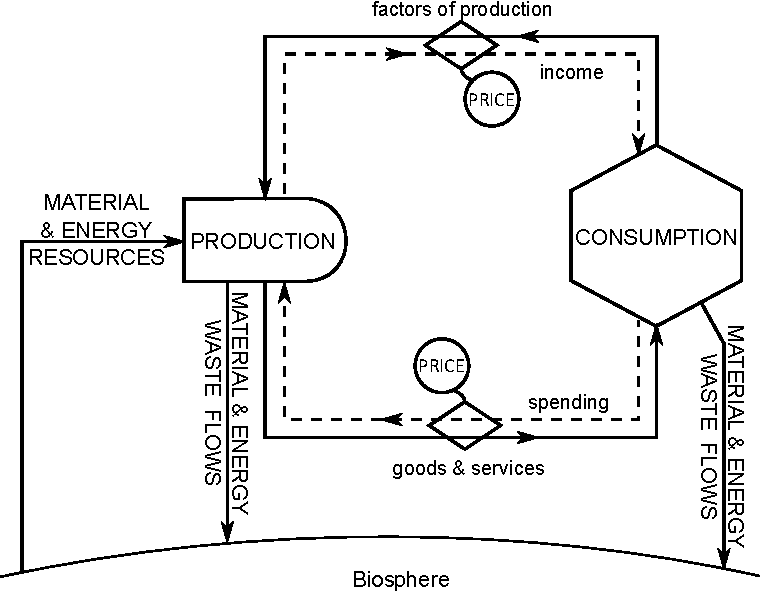
\includegraphics[width=\linewidth]{Part_0/Chapter_Acct_For_WoN/images/PERKS.pdf}
\caption[The metabolism model]{The metabolism model provides a comprehensive view 
of the economy, fully consistent with the laws of thermodynamics, 
including degraded resources (waste) expelled 
to the environment as a necessary consequence of economic activity.}
\label{fig:metabolic_economy}
\end{figure}

Although we're not the first to suggest the metabolism metaphor for the economy,
we believe that
the metabolism metaphor is underutilized 
on both practical and theoretical levels.
On the practical level, the metabolism metaphor is underutilized
because Systems of National Accounts, to date, 
are built upon the clockwork metaphor and traditional model for the economy
(Section~\ref{sec:era_of_energy_constraints}).
This book attempts to correct that oversight 
by using the metabolism metaphor 
to develop a rigorous theoretical framework 
for comprehensive national accounting.
(See Chapters~\ref{chap:materials}--\ref{chap:intensity}.)
On a theoretical level, the metabolism metaphor is underutilized, 
because, many researchers (with the exception of
the authors listed in Footnote~\ref{fn:metabolism_authors})
use the metabolism metaphor merely as as framing device for analyses of
raw material flows into the economy for the purpose of understanding 
stocks of raw materials in the biosphere.%
	\footnote{  %chktex 42
	The field most closely associated with the metabolism metaphor is
	Materials Flow Analysis (MFA). 
	To be fair, materials flow analysts clearly acknowledge that 
	materials flow into the economy (minerals and ores, especially),
	in part,
	for the purpose of building up stocks of technical infrastructure (buildings),
	livestock, and people.\cite[p.~116]{F-K1999} 
	However, there is little emphasis on quantifying \emph{levels} 
	of material stock in Materials \emph{Flow} Analysis, 
	as its name implies.
	In fact, the equations in MFA~\cite[Equation~1]{F-K1999} are almost always written as
	%
	\begin{equation*}
		\mathrm{inflow} = \mathrm{outflow} + \mathrm{accumulation \; ,}
	\end{equation*}
	%
	reflecting the focus on material inflow to the economy.
	In this book, similar equations 
	(see Equation~\ref{eq:general_accumulation_equation}) 
	are written as
	%
	\begin{equation*}
		\mathrm{accumulation} = \mathrm{inflow} - \mathrm{outflow \; ,}
	\end{equation*}
	%
	thereby focusing on accumulation of stocks within the economy.
	}
Some who employ the metabolism metaphor
tend to focus little attention on capital stock within the economy itself.
In effect, this is the same oversight as national accounting: 
under-appreciation of the important role of capital
in determining material and energy demand 
for its emplacement, use, maintenance, and replacement.

It becomes a vicious cycle. 
By not accounting for capital stock on a physical basis 
in national accounting, 
society is unable to appreciate 
the important physical role that capital stock plays in the economy
(Section~\ref{sec:stall_capital_stock}).
Because society under-appreciates the physical role of capital stock in the economy, 
there is little urgency to begin accounting 
for manufactured capital on a physical (rather than financial) basis.

We think that a deeper understanding of the metabolism metaphor
can serve to both highlight the important physical roles of both
resource extraction and manufactured capital stock and 
provide the basis for a rigorous theoretical framework 
for comprehensive national accounting.
In the following sections, 
we deepen the metabolism metaphor by considering 
anabolism (capital formation),
catabolism (energy production),
autophagy (recycling), and
issues of scale.%
	\footnote{  %chktex 42
	For the purposes of this discussion, 
	our focus is on metabolic processes as they occur 
	in eukaryotic animal cells 
	(cells with a nucleus containing genetic material), 
	thereby avoiding complexities associated 
	with organisms that also perform photosynthesis.
	}
Thereafter, we summarize the benefits of the metabolism metaphor
for national accounting.


%+++++++++ Anabolism ++++++++++
\subsection{Anabolism (capital formation)}
\label{sec:anabolism}
%+++++++++

Metabolic processes are classified as anabolic and catabolic 
(Section~\ref{sec:catabolism}).
Anabolic processes build up materials within the body 
(bones, muscles, and other tissues).
For example, anabolic steroids are hormones that stimulate 
the human body's natural muscle and bone growth processes.
Anabolic processes are fueled by the breakdown 
of adenosine triphosphate (ATP), the cellular energy source.
Raw materials for anabolic processes are provided by food, 
which, ultimately, comes from the biosphere.

The economic analog to biological anabolism is capital formation, 
net addition to the stock of capital (infrastructure, more generally) 
within a period of time.
Traditionally, capital formation is measured in currency units.
Thus, capital formation is the financial evidence 
of the emplacement of manufactured infrastructure.
Whereas biological anabolism is fueled by ATP, 
capital formation is fueled by the energy sector of the economy.
The raw material for capital formation comes to the 
economy from the biosphere.

We discuss extraction and use of materials in Chapter~\ref{chap:materials}
and the importance of capital stock throughout the book.


%+++++++++ Catabolism ++++++++++
\subsection{Catabolism (energy production)}
\label{sec:catabolism}
%+++++++++

Catabolic processes break down and destroy material stocks within an organism
through an oxidation process.
At the cellular level, catabolic oxidation releases chemical free energy, 
some of which synthesizes adenosine triphosphate (ATP), 
thereby providing fuel to cells. 
The remainder of the released energy is manifest as waste heat.
One of the waste products of cellular catabolism is CO$_2$.
Catabolic processes are part of a chain of material and energy transformations
wherein stored chemical energy is converted to useful energy
with waste heat and CO$_2$ as byproducts.

The analogy between catabolic processes and energy transformation processes
within the economy is striking.
Power plants (fired by coal, oil, natural gas, or refined liquid fuels) 
in either the energy sector or the final consumption sector
break down fossil fuels
in an oxidation process (combustion) to produce useful energy 
(typically, electricity or mechanical drive~\cite{Ayres:2010ug}), 
thereby providing energy to sectors of the economy.
Both waste heat and CO$_2$ are byproducts of combustion, 
and O$_2$ is consumed in the process.
Energy production in the economy is a chain of material and energy transformations 
wherein machines and engines 
convert stored chemical energy to useful energy
with waste heat and CO$_2$ as byproducts.

We focus on energy flows among sectors of the economy
in Chapter~\ref{chap:direct_energy}.


%+++++++++ Autophagy ++++++++++
\subsection{Autophagy (recycling)}
\label{sec:autophagy}
%+++++++++

One catabolic pathway, autophagy, 
involves the breakdown of damaged, unneeded, or dysfunctional cellular components 
(proteins and cell organelles)
for the purpose of re-use within the organism. 
Autophagy can be an adaptive response to low calorie intake,
promoting cell survival.

Again, the analogy between cellular metabolism and the economy is striking.
Whereas cellular autophagy repurposes proteins and cell organelles
for re-use by an organism,
recycling repurposes degraded
yet economically-valuable materials
for re-use by the economy.
Furthermore, recycling can also be an adaptive response 
to reduced material and energy inputs.
One famous example can be found on the streets of Cuba.
In the face of economic sanctions,
government restrictions on vehicle purchases, and
high import tariffs,
automobile imports by Cuba are very low.
As a result, Cuba hyper-recycles autos that were imported
prior to sanctions and manufactures replacement parts locally.
The average lifespan of automobiles has been extended
such that an estimated 60,000, pre-1960 cars~\cite{Schweid:2004aa} 
(so-called ``yank tanks'') are in service on the island.%
	\footnote{  %chktex 42
	Despite the recent change allowing new car purchases by individuals,
	astronomical import taxes mean that Cuban streets remain populated 
	with vintage 1950s autos.\cite{Ramey:2014aa}
	}
(See Figure~\ref{fig:vintage_autos_cuba}.)

\begin{figure}[!ht]
\centering\
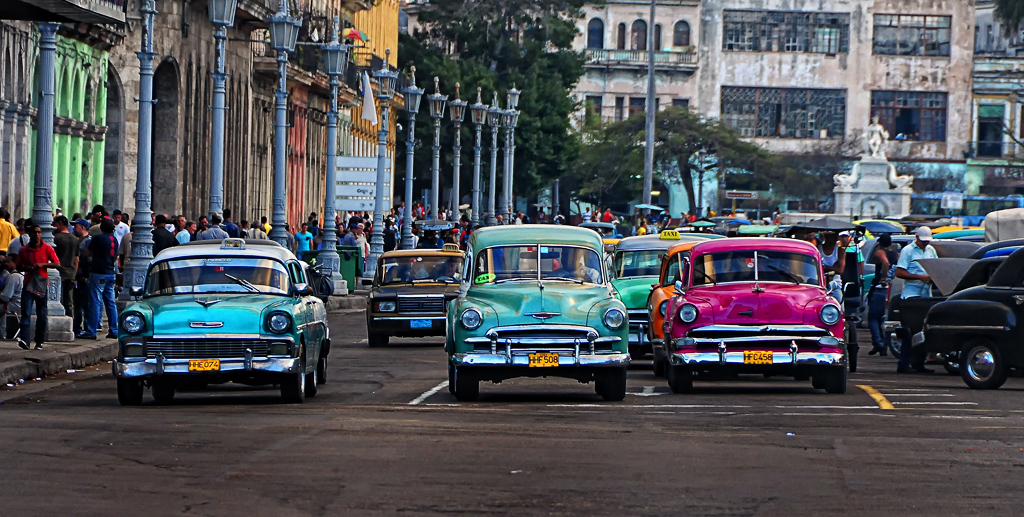
\includegraphics[width=\linewidth]{Part_0/Chapter_Acct_For_WoN/images/old-cars-of-cuba-dsc_4474-1024.jpg}  %chktex 8
\caption[Vintage autos in Cuba]{Vintage autos (``yank tanks'') in Cuba (2011).
**** \copyright~\emph{Larry Cowles, {\scriptsize \emph{\url{http://lcowlesphotography.wordpress.com}}}. Used by permission.} 
Permission not yet obtained. ****}
% This image is from
% \url{http://lcowlesphotography.wordpress.com/2011/02/13/old-cars-of-cuba/}.
% I emailed Larry Cowles to obtain permission to use the photo.
% See the Copyright Permissions folder for the email.
% If we can't obtain rights to Figure~\ref{fig:vintage_autos_cuba},
% other options include:
% \url{http://myadventuresacrosstheworld.wordpress.com/2013/03/14/transportation-in-cuba-old-cars-historical-cars-cocotaxi-bicitaxi-camionetas-and-what-not/}
% \url{http://www.travelforboomers.com/2012/10/17/so-close-and-yet-so-far-away-viva-cuba/}
% \url{http://ocean.otr.usm.edu/~w301497/travels/cuba2010/cuba2010b.html}
\label{fig:vintage_autos_cuba}
\end{figure}

It's not difficult to imagine that dynamics similar to Cuba's will emerge
if the inflow rate 
of any important natural but recyclable resource 
is reduced to a trickle
by the effects of depletion.%
	\footnote{  %chktex 42
	See Section~\ref{sec:stall_non-renewable_stocks}
	for a discussion of depletion of a non-recyclable natural resource, oil.	
	}

Regardless of the origin of material constraints, 
the effect on the economy will be the same:
re-use, recycling, and, where possible, substitution to other resources
will become increasingly imperative.

We focus on recycling in Section~\ref{sec:recycling}.


%+++++++++ Scale ++++++++++
\subsection{Issues of scale}
\label{sec:metabolic_scale}
%+++++++++

The metabolism metaphor brings to light issues of scale (size)
for economies and societies.
First, scale is directly related to material flow rates.
Larger organisms consume food at higher rates than smaller organisms,
in part to obtain essential nutrients to replenish cellular structures.
Similarly, economies with higher levels of emplaced capital
require larger material flow rates to provide 
raw materials to machines and food to people.
(See Section~\ref{sec:stall_capital_stock} for more on this topic.)

In Figure~\ref{fig:Kleiber_law},
we see Max Kleiber's empirically-determined relationship between
metabolic rate (heat production, in kcal/day) and
animal mass (in kg)
plotted on a log-log scale
for a variety of animals,
from mice to whales.
Dashed lines represent theoretical scaling due to either mass (weight)
or surface area.
The best fit to the data (thick line)
passes between the weight and surface area lines.

\begin{figure}[!ht]
\centering\
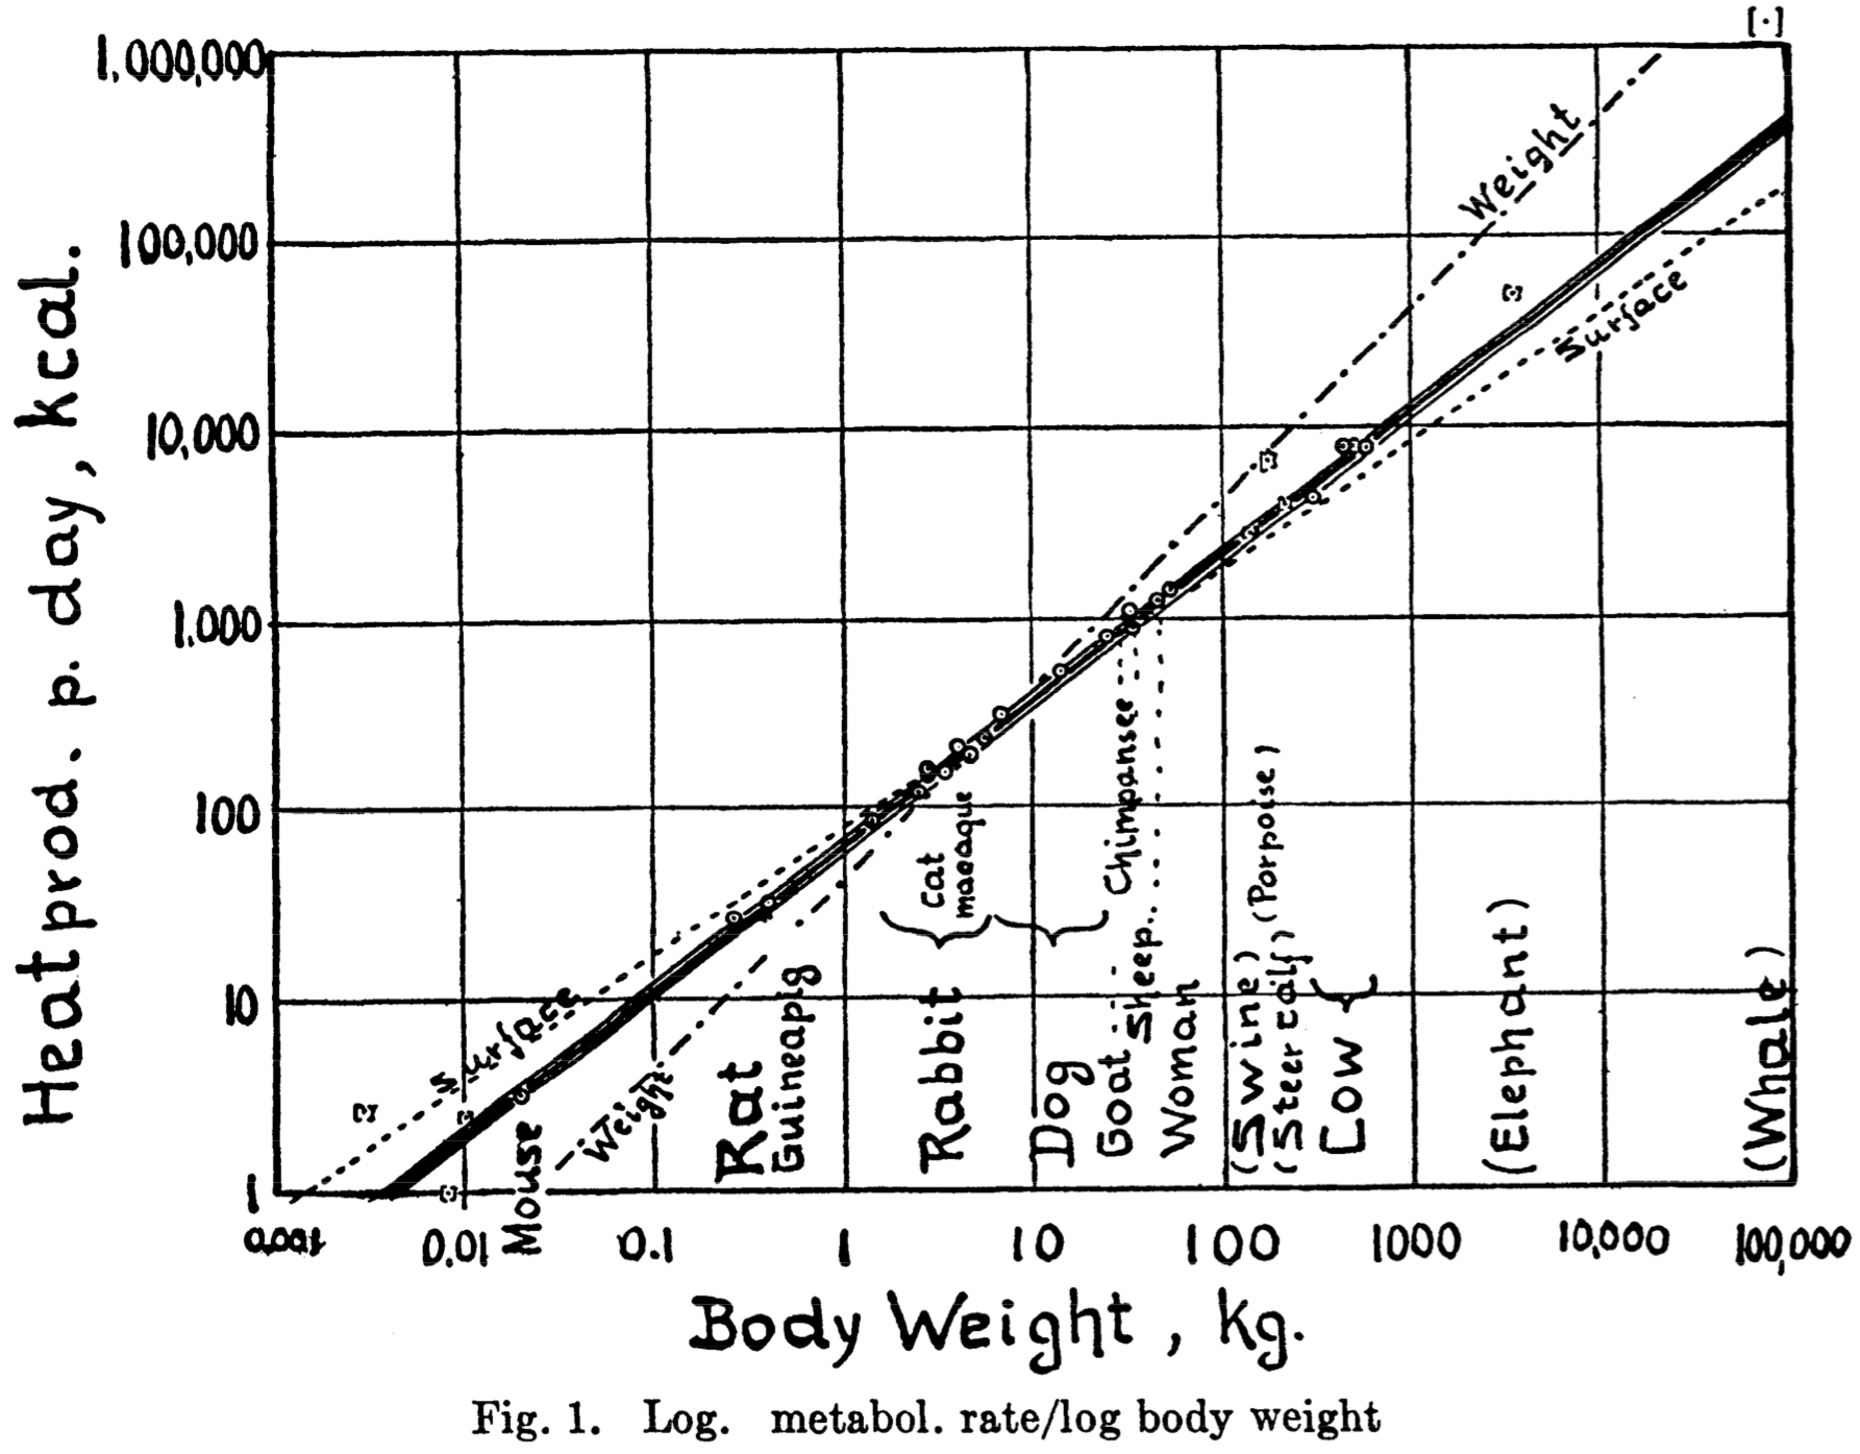
\includegraphics[width=\linewidth]{Part_0/Chapter_Acct_For_WoN/images/Kleiber1947.pdf}
\caption[Kleiber's law for metabolic rates of animals]{Kleiber's law 
for metabolic rates (heat production) of different-sized animals.\cite[p.~530]{Kleiber1947}
Larger animals, as determined by mass, have a higher metabolic rate, 
but the relationship between mass and metabolic rate is not linear.}
\label{fig:Kleiber_law}
\end{figure}

Kleiber's law which states this relationship mathematically,
is defined as
%
\begin{equation}\label{eq:Kleiber_law}
	\dot{Q} = q_{0} m^{\nicefrac{3}{4}}
\end{equation}
%
where 
$\dot{Q}$ is metabolic rate (heat production),
$m$ is the mass of the animal, and
$q_{0}$ is a mass-independent normalization constant.
From Equation~\ref{eq:Kleiber_law},
we see that doubling the mass increases the metabolic rate by
$2^{\nicefrac{3}{4}} = 1.68$ times.
To compensate for higher rates of heat loss due to high surface area-to-volume ratio,
small animals have higher metabolic rates
and larger food requirements per unit mass.%
	\footnote{  %chktex 42
	On a per-unit-mass basis, 
	Kleiber's Law becomes
	%
	\begin{equation}
		\frac{\dot{Q}}{m} = q_{0} m^{\nicefrac{-1}{4}} \; ,
	\end{equation}
	%
	from which it can be seen that 
	larger organisms (larger mass, $m$) consume less
	energy per unit mass~($\dot{Q}/m$), and 
	smaller organisms consume more
	energy per unit mass.
	}

If the economy is society's metabolism and 
the scale of an organism corresponds to the inventory 
of capital stock in an economy, 
the metabolism metaphor suggests that larger economies 
will require a higher rate of energy supply.
In fact, we know this to be true.
Built-out, industrialized economies with higher levels of emplaced capital
(those with more roads, cars, and buildings)
tend to consume energy at a higher rate, 
both in an absolute sense and on a per-capita basis,
compared to developing economies.


%%%%%%%%%% Metabolism metaphor helps %%%%%%%%%%
\subsection{Benefits of the metabolism metaphor}
\label{sec:metabolism_helps}
%%%%%%%%%%

The metabolism metaphor is compelling, 
because it helps us to see more clearly
and understand more deeply
how the real, biophysical economy operates.
But does the metabolism metaphor lead us to a better understanding 
of the coupling between the biosphere and the economy 
and provide guidance for more-comprehensive national accounting?
We think so.

In terms of a better understanding of the economy, 
the metabolism metaphor teaches us that the economy is a biophysical entity
that requires both materials and energy for survival.
We learn that economic activity is \emph{natural}.
It can be likened to breathing (respiration): 
O$_2$ is consumed as CO$_2$ is produced.
It can be likened to digestion:
raw materials and chemical potential energy are ingested, 
the body grows, 
and energy is provided for everyday activities.
Just as food from the biosphere provides materials and energy for
anabolic and catabolic processes in an organism, 
materials and fuels from the biosphere provide matter and energy for
capital formation and energy production in society.
Without materials and energy from the biosphere, 
metabolisms fail and organisms die. 
Without materials and energy from the biosphere,
the economies collapse and societies fade away.
In short, the economy is coupled to the biosphere,
because it is utterly and completely dependent upon it.

The metabolism metaphor teaches us that 
larger economies demand increasingly larger
material and energy flow rates from the biosphere.
We see that limits to economic growth
are both possible and expected.
From the metaphor we learn that economic ``stall'' is not pathological, 
but natural, especially in mature economies 
that have encountered some type of biophysical limit.
(See Section~\ref{sec:stall_non-renewable_stocks}.)
We might expect to encounter any number of limits:
supply rates of materials from the biosphere,
supply rates of energy from the biosphere,
scale of the economy relative to the biosphere.
In the metabolism metaphor, autophagy indicates that stocks 
of capital within society are reservoirs of 
material and (embodied) energy that can and should be 
broken down and re-used or re-purposed,
rather than discarded, 
when out of service.

Through an understanding of the deep interconnectedness and complexity
of organisms and species in the biosphere, 
we come to appreciate the interdependence 
among actors within and sectors of the economy.
Furthermore, an appreciation of the complex nature of economies leads us 
to acknowledge the difficulty in discerning
precisely which limit(s) is (are) encountered when growth stalls.  %chktex 36
In fact, there is no single explanation 
for the slowdown of growth in OECD economies 
discussed at the outset of Chapter~\ref{chap:intro}.
The best explanation to date involves many intertwining factors: 
slowing growth of energy input rate, 
decreasing energy return on investment in the liquid fuel sector,
problems in the credit markets, etc.

In terms of national accounting, 
a deeper understanding of the metabolism metaphor 
will lead to significant changes in national accounting.
It will lead us to acknowledge
the important role of \emph{both} flows 
(e.g., GDP, 
rates of material and energy extraction from the bioshere,
rates at which money spins through the economy)
\emph{and} stocks 
(e.g., manufactured capital, monetary savings, non-renewable energy supplies).
Furthermore, appreciation of the physical basis of the real economy will lead us 
to account for both stocks and flows 
in physical units (kg and kJ) as well as financial units (currency).

Deeper understanding of the metabolism metaphor will
lead systems of national accounts to become
focused as much on stocks as on flows.
Systems of national accounts will expand beyond financial accounting
to become a compendia of both physical as well as financial assets
of an economy.
By counting flows \emph{and} stocks 
in both physical and monetary units,
national accounting will provide a comprehensive picture 
of both the \emph{health} and the \emph{wealth} of economies, respectively.


%%%%%%%%%% New national accounting %%%%%%%%%%
\section{New national accounting}
\label{sec:new_national_accounting}
%%%%%%%%%%

Society needs to respond 
to the material and energy shortages that
we now face (Chapter~\ref{chap:intro}),
and part of that response
should involve more-comprehensive national accounting 
guided by a deeper understanding of the real, biophysical economy 
gained through the metabolism metaphor (Section~\ref{sec:economy_metabolism}).
It is imperative that we begin now
to help society deal with impending biophysical limits.

But how? 
What should we be counting and in what units?
And, how should the data be analyzed?



% *** Becky says - Matt - this next paragraph looks like
% it belongs in the last section of this chapter New
% national accounting. But I can't see how to
% fit it in. This is new and already in existence
% and in that chapter we talk
% about what is needed, so there is a mis-match.
% Could that section be changed a little to say that
% we heartily endorse the US expand its accounts to
% include something like SEEA. And, once it does,
% our framework could use that data to
% better understand the economy. What do you think?
% ***
% As described in the Prologue, the BEA has been prevented
% by political forces from developing accounts beyond
% financial flows of goods and services.
% Outside of the US, the international community has
% invested heavily in continued development
% of national accounting that accounts
% for the environment.
% The first System of National Accounts (SNA) was published by the UN
% soon after the US published its first set of national accounts.
% Since then, the UN has expanded the scope of the SNA to
% include interactions with the biosphere.
% The UN System of
% Environmental-Economic Accouting (SEEA) is a conceptual
% framework that was developed by a wide range
% of experts beginning in the early 1990s. This
% framework
% has just undergone a third, thorough
% revision using a global collaborative process.
% The SEEA are national accounts that
% capture data related to ``interactions between the
% economy and the environment, and the stocks
% and changes in stocks of environmental assets.''\cite[p. 1]{ UNSEEA2014}
% These accounts measure physical as well as financial flows, and are
% designed to dovetail with the SNA.

%**** Matt moved some of Becky's text here.
%	 Do we think it works?
%	
%	 For discussion:
%	
%	 The challenge is that we need to acknowledge that the SEEA exists.
%	
%	 We need to acknowledge that it is moving in the right direction.
%	
%	 We need to talk about its limitations honestly.
%	
%	 I'm not quite sure how to do this,
%	 because I know too little about the SEEA.
%	
%	 Is SEEA based on the metabolism metaphor?
%	
%	 Is SEEA as thorough as we think is needed?
%	
%	 Another approach could be to focus this on the US.
%	 We could say that the SEEA exists, but the US hasn't adopted yet.
%	 If the US is to move forward, it needs a firm theoretical grounding
%	 that doesn't exist at the SEEA.
%	 ****
%	
%	***** Mik--move this to Section 2.3. *****
%	A few countries (**** Say who they are? Or refer to Prologue. ****) 
%	are starting to include interactions 
%	between the biosphere and the economy in their national accounts,
%	guided by the UN's System of Environmental-Economic Accounting 
%	(SEEA).\cite[p. 1]{UNSEEA2014}.
%	We believe that a firm theoretical grounding
%	is needed for expanded Systems of National Accounts
%	that include interactions between the biosphere and the economy,
%	especially for inter-sector flows which are missing from the SEEA.
%	Also, material and capital accumulation within sectors.

%**** 
%Set up SEEA as the state of the art. 
%Use SEEA as launch point to say what additional is needed.
%Say how we relate to SEEA. 
%If this data were collected, this is another thing that could be done with it.
%Economy-wide information is a necessary first step to what we want to do.
%
%Possibly move footnote from p. 26 about SEEA to this location.
%****

As discussed in the Prologue, 
the UN System of Environmental-Economic Accouting (SEEA) 
is a conceptual framework 
that was developed by a wide range of experts 
beginning in the early 1990s. 
This framework has just undergone a third, 
thorough revision using a global collaborative process.
The SEEA are national accounts that
capture data related to ``interactions between the
economy and the environment, and the stocks
and changes in stocks of environmental assets.''~\cite[p. 1]{ UNSEEA2014}
These accounts measure physical as well as financial flows, and are
designed to dovetail with the SNA\@.
As such, the UN SEEA represents the state of the art,
in terms of accounting material and energy resource flows
through our economies.
If implemented, the SEEA allows national governments to answer questions
that were previously unknown,
such as, 
``At what rate do we use steel?'' or
``How much concrete is embodied within our economy?''
Indeed, analyses similar to the one presented in Figure~\ref{fig:Cleveland1984} 
(GDP vs.\ as a function of fuel consumption)
might be undertaken for any material (e.g., iron or water)
tracked by the SEEA\@.
Governments gain a great deal of understanding about the energetic
and material requirements of the country through the use of SEEA\@.

However, because the SEEA framework is defined at the economy-wide (E-W) scale,
there are many more important questions that still cannot be answered.
One such question is,
``What are the material and energetic requirements to scale up the renewable energy industry?''
This is a highly important question for future sustainable development,
not just for nations,
but for the globe as a whole.
Furthermore, the accumulation of materials and embodied energy
in the manufactured capital stock
of a particular economic sector is impossible to estimate with economy-wide analyses.
Such an analysis would require measuring inter-sectoral (i.e., intra-economy)
flows of materials and energy.
In the age of resource depletion, 
we believe obtaining inter-sectoral flows to be an essential
aspect of extended national accounting.

Firm theoretical grounding is needed 
\emph{before} we begin the process of expanding national accounts.
We need a framework, a way to organize our thoughts about the notion 
of national accounting in the age of resource depletion.
This book is an attempt to provide just that: 
a theoretical framework
for comprehensive national accounting
in the age of resource depletion
that could be adopted in systems of national accounts.

The first question above (``What should we be counting and in what units?'') 
is the topic for the remainder of this section,
and the answer provides the structure for the heart of the book.
The second question above (``How should the data be analyzed?'')
is the topic of Chapter~\ref{chap:intensity}.

We believe the key to understanding society's metabolism
in the age of resource depletion is to understand how 
materials, energy, embodied energy, and economic value
each interacts with the economy.
Specifically, it is important to understand how each
accumulates within the economy and how each flows into, within, and out of the economy.
The first three items (materials, energy, and embodied energy) are
inspired directly by the metabolism metaphor.
The fourth item (economic value) is necessary to understand the way 
that the lifeblood of economies (currency) flows through the economy.
Of course, each of the items in the list interacts with the others 
and the biosphere dynamically.
If we can begin to carefully track these items, 
we will be on our way toward gathering the information necessary to 
improve national accounting for the age of resource depletion.

National accounts that are informed by the metabolism metaphor 
and account for materials, energy, embodied energy, and economic value
may allow consumers, producers,
and policy-makers to answer critical questions that are not
answerable today, such as:

\begin{enumerate}
	\item{\textbf{How much energy was used in the manufacture and transport
				of two competing goods in the supermarket?} 
				(Or, equivalently, how much energy is embodied 
				in two competing goods in the supermarket?)}
	\item{\textbf{What might be the optimal scale of an economy in terms of GDP 
				and what are the impacts of an optimally-sized economy on natural capital?}}
    \item{\textbf{How is is dependence upon scarce fossil fuels embedded 
    			in the interwoven fabric of the economy?}} 
    \item{\textbf{How will economies that are dependent on coal, oil, 
     			and other forms of non-renewable energy transition 
    			to renewable forms of energy?}}
	\item{\textbf{How might an economy be affected as an increasing share of production
				is directed toward replacing 
				degraded ecosystem services?}~\cite[p.~221]{kummel2011}​}
	\item{\textbf{What are the material and energy requirements to scale up 
				the renewable energy industry?}}
\end{enumerate}

Our approach to developing a rigorous theoretical foundation for 
comprehensive national accounting is to
develop a dynamic model 
by applying rigorous thermodynamics 
to materials and energy flows into, among, 
and out of economic sectors,
informed by the metabolism metaphor,
in a manner that is verifiable against 
the existing (or expanded) 
national accounts.


%%%%%%%%%% Structure %%%%%%%%%%
\section{Structure of the book}
\label{sec:structure}
%%%%%%%%%%

The list of items to be accounted 
(materials, energy, embodied energy, and economic value)
provides structure for our proposed framework
and much of the rest of this book.

Part~\ref{part:matter} addresses flows of physical matter and energy
through the economy.
Chapter~\ref{chap:materials} discusses material flows and accumulation.
Flows of energy are covered in Chapter~\ref{chap:direct_energy}, 
and a rigorous, thermodynamics-based definition of and accounting for 
embodied energy is presented in Chapter~\ref{chap:embodied_energy}.

In Part~\ref{part:values}, we turn to flow and accumulation of 
non-physical entities through the economy. 
Flows and accumulation of economic value are discussed in Chapter~\ref{chap:value}.
In Chapter~\ref{chap:intensity}, we combine the results from 
Chapters~\ref{chap:embodied_energy} and~\ref{chap:value} to
develop an important indicator of economic activity:
the energy intensity of economic production.

Part~\ref{part:implications} gives context to the framework developed in
Parts~\ref{part:matter}~and~\ref{part:values}.
Chapter~\ref{chap:implications} draws out some of the direct implications
of our model.
And, we end with a summary and a proposed list of next steps in Chapter~\ref{chap:summary}.

Throughout the methodological chapters~(\ref{chap:materials}--\ref{chap:intensity}),
our accounting framework is developed
through a series of increasingly-disaggregated
models of the economy~(Table~\ref{tab:examplesABC})
using, as much as possible, the same structure for each.
Doing so provides a detailed, step-by-step explanation of our proposed accounting framework.
We use the US auto industry 
as a running example for application and discussion.

\begin{table}
\caption[Examples used throughout this book]{Examples
used throughout this book.}
\begin{center}
  \begin{tabular}{c @{\hspace{1.5em}} c @{\hspace{1.5em}} c @{\hspace{1.5em}} c @{\hspace{1.5em}} c}
    \toprule
    Example & Sector 0 & Sector 1 & Sector 2 & Sector 3 \\ 
	\midrule
    A & Biosphere	&	Society            & NA         & NA                 \\
    B & Biosphere	&	Final Consumption  & Production & NA                 \\
    C & Biosphere	&	Final Consumption  & Energy     & Goods \& Services  \\
  \bottomrule
  \end{tabular}
\end{center}
\label{tab:examplesABC}
\end{table}
 

\bibliographystyle{unsrt}
\bibliography{../../Metabolic}  %chktex 11






%%%%%%%%%%%%%%%%%%%%%%%%%%%%%%%%%%%%%%%%
%%%%%%%%%%%%%%%%%%%%%%%%%%%%%%%%%%%%%%%%
% BONEPILE
%%%%%%%%%%%%%%%%%%%%%%%%%%%%%%%%%%%%%%%%
%%%%%%%%%%%%%%%%%%%%%%%%%%%%%%%%%%%%%%%%

% %%%%%%%%%% Metaphors and Models %%%%%%%%%%
% \section{Metaphors and models}
% \label{sec:metaphors_and_models}
% %%%%%%%%%%
%
% As discussed in Section~\ref{sec:new_accounting},
% national accounting is incomplete, and
% an objective for this book is to provide rigorous theoretical grounding for
% a better national accounting framework.
%
% **** The motivation for this comes from looking at the history
% of how society has determined what should be incuded in national accounts.
% Change the
%
% The need for this is obvious when we look the vision society has for national accounts.
% ****
%
% But, before moving ahead with developing that framework,
% it is useful to consider how society has come to this point.
% How is it that we don't routinely and comprehensively account for
% important material and energy flows into, within, and out of the economy
% on a physical basis in systems of national accounts?
%
% The classical economists certainly appreciated the dependence of
% economic activity on biophysical processes.\cite{Hall2011, Cleveland1987, Dale2012}
% However, somewhere between William Stanley Jevons' 1865
% assessment that
% ``the very existence of Britain, as a great nation''~\cite[IV.3]{Jevons1865}
% was tied to a continued supply of low-cost coal
% and Julian Simon's 1998 statement that
% ``natural resources are not finite in any economic sense,''~\cite[p.~54]{Simon1998} %chktex 38
% the importance of the biosphere was lost.
% In the following sections, we argue that
% a contributing reason for incomplete national accounting
% is that we have the wrong metaphor for the economy,
% and we provide a suggestion for improvement.
%
%
% %+++++++++ The clockwork metaphor ++++++++++
% \subsection{The clockwork metaphor}
% \label{sec:clockwork_metaphor}
% %+++++++++
%
% Most economics textbooks today depict the economy
% as in Figure~\ref{fig:perp_motion_1}.
% Goods and services flow from the production sector
% to the household sector~(consumption)
% in exchange for payments.
% The factors of production (labor and capital)
% flow from the household sector to the
% production sector in exchange for wages and rents (income).
% Attention is primarily focused on the circular flow
% of money~(dashed line).
%
% \begin{figure}[!ht]
% \centering\
% \includegraphics[width=\linewidth]{Part_0/Chapter_Introduction/images/Perpetual_motion_1.pdf}
% \caption[The traditional model]{In the traditional model, the economy
% is represented as a circular flow of goods and services between two sectors.
% Producers manufacture goods and services
% by taking in labor and capital.
% Consumers exchange labor for wages
% which are used to purchase
% the goods and services of the producers.}
% \label{fig:perp_motion_1}
% \end{figure}
%
% This traditional model of the economy~(Figure~\ref{fig:perp_motion_1})
% is unashamedly mechanistic.
% General equilibrium models of the economy
% ~\cite{Walras1892, Walras1993}
% were borrowed directly from classical physics' models of
% mechanical equilibrium which, in turn, arose from the
% ``clockwork universe'' metaphor.\cite{Ingrao1990}
% The clockwork metaphor is a simplification
% that helps us make sense of the world around us.
% Like all metaphors, it informs our thinking about the real world,
% but, consequently,
% it also constrains our ability to frame reality.
% Erroneously, we mistake the model-metaphor for reality, and
% we interact with reality in the same manner
% as we interact with the abstract objects of our
% models.\footnote{This fallacious process is known as
% 	\emph{reification}; the making (\emph{facere}, Latin) real of
% 	something (\emph{res}, Latin) that is merely an idea.
% 	Alfred Whitehead refers to this as
% 	\emph{the fallacy of misplaced concreteness}.\cite{Whitehead2011}
% 	}
% Classical physics told us the universe was
% \emph{like} clockwork,
% so we began to interact with the universe
% as if it \emph{really were} clockwork.
% It then became easy to collect economic data that confirmed the clockwork model,
% because the model told us which data to collect.
%
% The clockwork metaphor and the traditional model of the economy
% preclude any sort of connection
% between the economy and the biosphere.
% Thus, only the internal dynamics of the economy are important.
% They tell us that natural resources are unimportant,
% effectively assuming that the biosphere will always provide.
% If a particular resource becomes scarce,
% substitution to a different, more-readily-available resource will be made.
% Wastes are quantitatively unimportant,
% effectively assuming that the biosphere has infinite assimilative capacity.
% Economic forces (through prices and the market mechanism)
% are thought to effectively guide any necessary transition
% within the economy.
% With the clockwork metaphor, physical constraints
% imposed by the biosphere
% on allocation of resources, distribution of outputs, and
% scale of an economy
% are outside the scope of neoclassical economic discussion.\cite{Daly1995}
% In short, the clockwork metaphor and the traditional model of the economy
% tell us that the clockwork-economy can and will carry on.
%
% In light of the discussion in Chapter~\ref{chap:intro},
% the clockwork metaphor and traditional model of the economy
% are clearly problematic.
% Because Figure~\ref{fig:perp_motion_1} has no flow of energy
% into the economy,
% we may consider the traditional model of the economy
% to be a perpetual motion machine of the \emph{first kind}:
% the economy works without the input of energy, thus violating
% the First Law of Thermodynamics---the
% law of conservation of energy.\cite{Rao2004}
%
%
% %%%%%%%%%% Machine metaphor %%%%%%%%%%
% \subsection{The machine metaphor}
% \label{sec:machine_metaphor}
% %%%%%%%%%%
%
% The limits of the clockwork metaphor and traditional model of the economy were
% exposed by the oil shocks of the 1970s.
% The global economy
% ``stalled'' due to lack of
% a single, highly-constrained resource:
% fuel.
% Many came to realize that input energy is required
% for successful operation of an economic ``engine.''
% Thus, a machine metaphor and
% accompanying engine model for the economy
% rose to prominence
% in the late 1970s and early 1980s.
% The need to include energy resources
% in the economic picture
% spurred the efforts of early (net) energy
% analysts.\cite{Gilliland1975, Chapman1976}
%
% The engine model (Figure~\ref{fig:perp_motion_2})
% accounts for energy flows from the biosphere
% to the economy.
% With the new metaphor, the economy changed from
% an \emph{isolated} system~(Figure~\ref{fig:perp_motion_1}) to
% a \emph{closed} system~(Figure~\ref{fig:perp_motion_2}).
% The importance of input energy was acknowledged,
% but wastes are missing.
% And, the biosphere is relegated to the position
% of provider of energy resources;
% the larder and gas station of the economy.\cite{Norgaard2010}
%
% \begin{figure}[H]
% \centering\
% \includegraphics[width=\linewidth]{Part_0/Chapter_Introduction/images/Perpetual_motion_2.pdf}
% \caption[The machine model]{The machine model of the economy includes
% flows of energy into the economy from the biosphere.
% This may be considered a perpetual motion machine
% of the second kind.}
% \label{fig:perp_motion_2}
% \end{figure}
%
% The machine metaphor and engine model,
% like the clockwork metaphor and traditional model,
% are mechanistic.
% Much like the engines of the Industrial Revolution,
% the economic engine is assumed to be well-behaved and amenable to control.
% Even today, machine metaphors abound in our economic discussions.
% We continue to speak of ``fueling'' the ``economic engine''
% lest it should ``stall.''~\cite{Liu2012}
% Like a well-running engine, the economy is assumed
% to be resilient to small or even quite large perturbations.
% It can either self-correct,
% or be corrected predictably with adjustments to
% a few policy levers.
%
% But how accurate is the engine model?
%
% According to the Second Law of Thermodynamics,
% all real-world processes involve the degradation
% of material and, especially, energy resources
% and the creation of entropy.
% High quality (low entropy) material and energy come in;
% low quality (high entropy) material and energy go out.
% Wastes exist!
% The depiction of the economy in Figure~\ref{fig:perp_motion_2}
% can be classified as a perpetual motion machine
% of the \emph{second kind}:
% it perfectly converts energy resources into
% work~(useful energy services) without generating
% any entropy,
% in violation of the Second Law of Thermodynamics.
% Because the generation of high entropy~(low quality)
% output is a \emph{necessary} feature of \emph{all} processes
% (including economic processes),
% the generation of wastes is a \emph{normal} feature of
% the economy,
% not an anomaly.
%
% None of the clockwork metaphor, the traditional model,
% the machine metaphor, or the engine model
% is sufficient to describe a real economy.
%
% We need a different model.
%
% We need a new metaphor.



% Always give a unique label
% and use \ref{<label>} for cross-references
% and \cite{<label>} for bibliographic references
% use \sectionmark{}
% to alter or adjust the section heading in the running head
%% Instead of simply listing headings of different levels we recommend to let every heading be followed by at least a short passage of text. Furtheron please use the \LaTeX\ automatism for all your cross-references and citations.

%% Please note that the first line of text that follows a heading is not indented, whereas the first lines of all sequent paragraphs are.

%% Use the standard \verb|equation| environment to typeset your equations, e.g.
%
%% \begin{equation}
%% a \times b = c\;,
%% \end{equation}
%
%% however, for multiline equations we recommend to use the \verb|eqnarray|
%% environment\footnote{In physics texts please activate the class option \texttt{vecphys} to depict your vectors in \textbf{\itshape boldface-italic} type - as is customary for a wide range of physical jects.}.
%% \begin{eqnarray}
%% a \times b = c \nonumber\\
%% \vec{a} \cdot \vec{b}=\vec{c}
%% \label{eq:01}
%% \end{eqnarray}

%% \section{section Heading}
%% \label{sec:2}
%% Instead of simply listing headings of different levels we recommend to let every heading be followed by at least a short passage of text. Furtheron please use the \LaTeX\ automatism for all your cross-references\index{cross-references} and citations\index{citations} as has already been described in Sect.~\ref{sec:2}.

%% \begin{quotation}
%% Please do not use quotation marks when quoting texts! Simply use the \verb|quotation| environment -- it will automatically render Springer's preferred layout.
%% \end{quotation}


%% \section{section Heading}
%% Instead of simply listing headings of different levels we recommend to let every heading be followed by at least a short passage of text. Furtheron please use the \LaTeX\ automatism for all your cross-references and citations as has already been described in Sect.~\ref{sec:2}, see also Fig.~\ref{fig:1}\footnote{If you copy text passages, figures, or tables from other works, you must obtain \textit{permission} from the copyright holder (usually the original publisher). Please enclose the signed permission with the manucript. The sources\index{permission to print} must be acknowledged either in the captions, as footnotes or in a separate section of the book.}

%% Please note that the first line of text that follows a heading is not indented, whereas the first lines of all sequent paragraphs are.

% For figures use
%
%% \begin{figure}[b]
%% \sidecaption
% Use the relevant command for your figure-insertion program
% to insert the figure file.
% For example, with the option graphics use
%% \includegraphics[scale=.65]{figure}
%
% If not, use
%\picplace{5cm}{2cm} % Give the correct figure height and width in cm
%
%% \caption{If the width of the figure is less than 7.8 cm use the \texttt{sidecapion} command to flush the caption on the left side of the page. If the figure is positioned at the top of the page, align the sidecaption with the top of the figure -- to achieve this you simply need to use the optional argument \texttt{[t]} with the \texttt{sidecaption} command}
%% \label{fig:1}       % Give a unique label
%% \end{figure}


%% \paragraph{Paragraph Heading} %
%% Instead of simply listing headings of different levels we recommend to let every heading be followed by at least a short passage of text. Furtheron please use the \LaTeX\ automatism for all your cross-references and citations as has already been described in Sect.~\ref{sec:2}.

%% Please note that the first line of text that follows a heading is not indented, whereas the first lines of all sequent paragraphs are.

%% For typesetting numbered lists we recommend to use the \verb|enumerate| environment -- it will automatically render Springer's preferred layout.

%% \begin{enumerate}
%% \item{Livelihood and survival mobility are oftentimes coutcomes of uneven socioeconomic development.}
%% \begin{enumerate}
%% \item{Livelihood and survival mobility are oftentimes coutcomes of uneven socioeconomic development.}
%% \item{Livelihood and survival mobility are oftentimes coutcomes of uneven socioeconomic development.}
%% \end{enumerate}
%% \item{Livelihood and survival mobility are oftentimes coutcomes of uneven socioeconomic development.}
%% \end{enumerate}


%% \paragraph{paragraph Heading} In order to avoid simply listing headings of different levels we recommend to let every heading be followed by at least a short passage of text. Use the \LaTeX\ automatism for all your cross-references and citations as has already been described in Sect.~\ref{sec:2}, see also Fig.~\ref{fig:2}.

%% Please note that the first line of text that follows a heading is not indented, whereas the first lines of all sequent paragraphs are.

%% For unnumbered list we recommend to use the \verb|itemize| environment -- it will automatically render Springer's preferred layout.

%% \begin{itemize}
%% \item{Livelihood and survival mobility are oftentimes coutcomes of uneven socioeconomic development, cf. Table~\ref{tab:1}.}
%% \begin{itemize}
%% \item{Livelihood and survival mobility are oftentimes coutcomes of uneven socioeconomic development.}
%% \item{Livelihood and survival mobility are oftentimes coutcomes of uneven socioeconomic development.}
%% \end{itemize}
%% \item{Livelihood and survival mobility are oftentimes coutcomes of uneven socioeconomic development.}
%% \end{itemize}

%% \begin{figure}[t]
%% \sidecaption[t]
% Use the relevant command for your figure-insertion program
% to insert the figure file.
% For example, with the option graphics use
%% \includegraphics[scale=.65]{figure}
%
% If not, use
%\picplace{5cm}{2cm} % Give the correct figure height and width in cm
%
%% \caption{Please write your figure caption here}
%% \label{fig:2}       % Give a unique label
%% \end{figure}

%% \runinhead{Run-in Heading Boldface Version} Use the \LaTeX\ automatism for all your cross-references and citations as has already been described in Sect.~\ref{sec:2}.

%% \runinhead{Run-in Heading Italic Version} Use the \LaTeX\ automatism for all your cross-refer\-ences and citations as has already been described in Sect.~\ref{sec:2}\index{paragraph}.
% Use the \index{} command to code your index words
%
% For tables use
%
%% \begin{table}
%% \caption{Please write your table caption here}
%% \label{tab:1}       % Give a unique label
%
% For LaTeX tables use
%
%% \begin{tabular}{p{2cm}p{2.4cm}p{2cm}p{4.9cm}}
%% \hline\noalign{\smallskip}
%% Classes & class & Length & Action Mechanism  \\
%% \noalign{\smallskip}\svhline\noalign{\smallskip}
%% Translation & mRNA$^a$  & 22 (19--25) & Translation repression, mRNA cleavage\\
%% Translation & mRNA cleavage & 21 & mRNA cleavage\\
%% Translation & mRNA  & 21--22 & mRNA cleavage\\
%%Translation & mRNA  & 24--26 & Histone and DNA Modification\\
%%\noalign{\smallskip}\hline\noalign{\smallskip}
%%\end{tabular}
%%$^a$ Table foot note (with superscript)
%%\end{table}
%
%% \section{Section Heading}
%%\label{sec:3}
% Always give a unique label
% and use \ref{<label>} for cross-references
% and \cite{<label>} for bibliographic references
% use \sectionmark{}
% to alter or adjust the section heading in the running head
%% Instead of simply listing headings of different levels we recommend to let every heading be followed by at least a short passage of text. Furtheron please use the \LaTeX\ automatism for all your cross-references and citations as has already been described in Sect.~\ref{sec:2}.

%% Please note that the first line of text that follows a heading is not indented, whereas the first lines of all sequent paragraphs are.

%%If you want to list definitions or the like we recommend to use the Springer-enhanced \verb|description| environment -- it will automatically render Springer's preferred layout.

%%\begin{description}[Type 1]
%%\item[Type 1]{That addresses central themes pertainng to migration, health, and disease. In Sect.~\ref{sec:1}, Wilson discusses the role of human migration in infectious disease distributions and patterns.}
%%\item[Type 2]{That addresses central themes pertainng to migration, health, and disease. In Sect.~\ref{sec:2}, Wilson discusses the role of human migration in infectious disease distributions and patterns.}
%%\end{description}

%%\section{section Heading} %
%% In order to avoid simply listing headings of different levels we recommend to let every heading be followed by at least a short passage of text. Use the \LaTeX\ automatism for all your cross-references and citations citations as has already been described in Sect.~\ref{sec:2}.

%% Please note that the first line of text that follows a heading is not indented, whereas the first lines of all sequent paragraphs are.

%% \begin{svgraybox}
%% If you want to emphasize complete paragraphs of texts we recommend to use the newly defined Springer class option \verb|graybox| and the newly defined environment \verb|svgraybox|. This will produce a 15 percent screened box 'behind' your text.

%% If you want to emphasize complete paragraphs of texts we recommend to use the newly defined Springer class option and environment \verb|svgraybox|. This will produce a 15 percent screened box 'behind' your text.
%% \end{svgraybox}


%% \section{section Heading}
%%Instead of simply listing headings of different levels we recommend to let every heading be followed by at least a short passage of text. Furtheron please use the \LaTeX\ automatism for all your cross-references and citations as has already been described in Sect.~\ref{sec:2}.

%% Please note that the first line of text that follows a heading is not indented, whereas the first lines of all sequent paragraphs are.

%% \begin{theorem}
%% Theorem text goes here.
%% \end{theorem}
%
% or
%
%% \begin{definition}
%% Definition text goes here.
%% \end{definition}

%% \begin{proof}
%\smartqed
%% Proof text goes here.
%% \qed
%% \end{proof}

%%\paragraph{Paragraph Heading} %
%% Instead of simply listing headings of different levels we recommend to let every heading be followed by at least a short passage of text. Furtheron please use the \LaTeX\ automatism for all your cross-references and citations as has already been described in Sect.~\ref{sec:2}.

%% Note that the first line of text that follows a heading is not indented, whereas the first lines of all subsequent paragraphs are.
%
% For built-in environments use
%
%%\begin{theorem}
%%Theorem text goes here.
%%\end{theorem}
%
%%\begin{definition}
%%Definition text goes here.
%%\end{definition}
%
%%\begin{proof}
%%\smartqed
%% Proof text goes here.
%%\qed
%%\end{proof}
%
%% \begin{acknowledgement}
%% If you want to include acknowledgments of assistance and the like at the end of an individual chapter please use the \verb|acknowledgement| environment -- it will automatically render Springer's preferred layout.
%% \end{acknowledgement}
%
%% \section*{Appendix}
%% \addcontentsline{toc}{section}{Appendix}
%
%% When placed at the end of a chapter or contribution (as opposed to at the end of the book), the numbering of tables, figures, and equations in the appendix section continues on from that in the main text. Hence please \textit{do not} use the \verb|appendix| command when writing an appendix at the end of your chapter or contribution. If there is only one the appendix is designated ``Appendix'', or ``Appendix 1'', or ``Appendix 2'', etc. if there is more than one.

%% \begin{equation}
%% a \times b = c
%% \end{equation}
% Problems or Exercises should be sorted chapterwise
%% \section*{Problems}
%% \addcontentsline{toc}{section}{Problems}
%
% Use the following environment.
% Don't forget to label each problem;
% the label is needed for the solutions' environment
%% \begin{prob}
%% \label{prob1}
%% A given problem or Excercise is described here. The
%% problem is described here. The problem is described here.
%% \end{prob}

%% \begin{prob}
%% \label{prob2}
%% \textbf{Problem Heading}\\
%% (a) The first part of the problem is described here.\\
%% (b) The second part of the problem is described here.
%% \end{prob}


